\subsection{逻辑回归}\label{sec:12.3}
\autoref{sec:11.3.3}的条件正态模型是广义线性模型（GLM）的一个例子. GLM描述响应变量$Y$的均值与自变量$x$之间的关系，但这种关系可能比\eqref{eq:11.3.2}的$EY_i=\alpha+\beta x_i$更复杂. 许多不同模型都可表示为GLM. 本节专门讨论一种GLM：逻辑回归模型.

\subsubsection{模型}\label{sec:12.3.1}
GLM由三部分组成：随机成分、系统成分和连接函数.
\begin{enumerate}[label=(\arabic*)]
\item 响应变量$Y_1,\ldots,Y_n$是随机成分（random component）. 假定它们相互独立，各自的分布都属于指定的指数族. 各$Y_i$不同分布，但都属于同一个分布族，如二项、Poisson、正态等.
\item 系统成分（systematic component）就是模型. 它是预测变量$x_i$的函数，对参数为线性，并与$Y_i$的均值有关. 例如，系统成分可以是$\alpha+\beta x_i$或$\alpha+\beta/x_i$. 这里只考虑$\alpha+\beta x_i$.
\item 最后，连接函数（link function）$g(\mu)$通过规定$g(\mu_i)=\alpha+\beta x_i$联系这两部分，其中$\mu_i=EY_i$.
\end{enumerate}

\sourcepageanchor{510}
\autoref{sec:11.3.3}的条件正态回归模型就是GLM. 在该模型中，各响应$Y_i$都服从正态分布. 正态族当然是指数族，构成随机成分. 回归函数的形式为$\alpha+\beta x_i$，这就是系统成分. 最后，假设关系$\mu_i=EY_i=\alpha+\beta x_i$，意味着连接函数为$g(\mu)=\mu$. 这个简单连接函数称为恒等连接（identity link）.

另一个很有用的GLM是逻辑回归模型. 此时响应$Y_1,\ldots,Y_n$相互独立，$Y_i\sim\operatorname{Bernoulli}(\pi_i)$. （Bernoulli族是指数族.）回顾$EY_i=\pi_i=P(Y_i=1)$. 在这一模型中，假定$\pi_i$与$x_i$满足
\begin{equation}\label{eq:12.3.1}
\log\left(\frac{\pi_i}{1-\pi_i}\right)=\alpha+\beta x_i.
\end{equation}
左边是$Y_i$成功的优势（odds）的对数. 模型假定这一对数优势（log-odds，或logit）是预测变量$x$的线性函数. Bernoulli的pmf可写成指数族形式
$$\pi^y(1-\pi)^{1-y}=(1-\pi)\exp\left\{y\log\left(\frac{\pi_i}{1-\pi_i}\right)\right\}.$$
$\log(\pi/(1-\pi))$是这个指数族的自然参数，\eqref{eq:12.3.1}采用连接函数$g(\pi)=\log(\pi/(1-\pi))$. 以这种方式使用自然参数时，称为典范连接（canonical link）.

\eqref{eq:12.3.1}可改写为
$$\pi_i=\frac{e^{\alpha+\beta x_i}}{1+e^{\alpha+\beta x_i}},$$
或更一般地，
\begin{equation}\label{eq:12.3.2}
\pi(x)=\frac{e^{\alpha+\beta x}}{1+e^{\alpha+\beta x}}.
\end{equation}
可见$0<\pi(x)<1$，由于$\pi(x)$是概率，这似乎合理. 但若某些$x$可能有$\pi(x)=0$或1，这个模型就不适用. 更仔细地考察$\pi(x)$，其导数可写为
\begin{equation}\label{eq:12.3.3}
\frac{d\pi(x)}{dx}=\beta\pi(x)(1-\pi(x)).
\end{equation}
因为$\pi(x)(1-\pi(x))$始终为正，$\pi(x)$的导数随$\beta$为正、零、负而分别为正、零、负. 若$\beta>0$，$\pi(x)$关于$x$严格递增；若$\beta<0$，则严格递减. 若$\beta=0$，对所有$x$有$\pi(x)=e^\alpha/(1+e^\alpha)$. 与简单线性回归一样，$\beta=0$表示$\pi$与$x$之间没有关系. 此外，在逻辑回归模型中，$\pi(-\alpha/\beta)=1/2$. 逻辑回归函数具有如下对称性：对任意$c$，$\pi((-\alpha/\beta)+c)=1-\pi((-\alpha/\beta)-c)$.

参数$\alpha,\beta$的含义与简单线性回归相似. 在\eqref{eq:12.3.1}中令$x=0$，得$\alpha$是$x=0$时成功的对数优势. 分别在$x,x+1$处计算\eqref{eq:12.3.1}，对任意$x$有
$$\log\left(\frac{\pi(x+1)}{1-\pi(x+1)}\right)-\log\left(\frac{\pi(x)}{1-\pi(x)}\right)
=\alpha+\beta(x+1)-\alpha-\beta(x)=\beta.$$
所以$\beta$是$x$增加一个单位所对应的成功对数优势变化量. 简单线性回归中，$\beta$是$x$增加一个单位所对应的$Y$均值变化量. 对等式两边取指数得到
\begin{equation}\label{eq:12.3.4}
e^\beta=\frac{\pi(x+1)/(1-\pi(x+1))}{\pi(x)/(1-\pi(x))}.
\end{equation}
\sourcepageanchor{511}
右边是比较$x+1$与$x$处成功优势的优势比（odds ratio）. （回顾\autoref{ex:5.5.19}和\autoref{ex:5.5.22}讨论过优势的估计.）逻辑回归模型中，这个比值作为$x$的函数为常数. 最后，
\begin{equation}\label{eq:12.3.5}
\frac{\pi(x+1)}{1-\pi(x+1)}=e^\beta\frac{\pi(x)}{1-\pi(x)};
\end{equation}
即$e^\beta$是$x$增加一个单位所对应的成功优势的乘法变化因子.

\eqref{eq:12.3.2}提示了将Bernoulli成功概率$\pi(x)$建模为预测变量$x$的函数的其他方法. 回顾$F(w)=e^w/(1+e^w)$是logistic$(0,1)$分布的cdf. 在\eqref{eq:12.3.2}中假定$\pi(x)=F(\alpha+\beta x)$. 使用其他连续cdf可定义$\pi(x)$的其他模型. 若$F(w)$为标准正态cdf，称为probit回归（probit regression，见\autoref{exercise:12.17}）. 若采用Gumbel的cdf，连接函数称为log-log连接.

\subsubsection{估计}\label{sec:12.3.2}
在线性回归中，采用$Y_i=\alpha+\beta x_i+\varepsilon_i$这样的模型时，可以选择最小二乘方法计算$\alpha,\beta$的估计. 这里已不再如此. 在模型\eqref{eq:12.3.1}中，$Y_i\sim\operatorname{Bernoulli}(\pi_i)$，$Y_i$与$\alpha+\beta x_i$不再直接相连，这也正是需要连接函数的原因. 因而，最小二乘已不再是一种选择.

最常用的估计方法是最大似然. 一般模型为$Y_i\sim\operatorname{Bernoulli}(\pi_i)$，其中$\pi(x)=F(\alpha+\beta x)$. 若记$F_i=F(\alpha+\beta x_i)$，似然函数为
$$L(\alpha,\beta\mid\boldsymbol y)=\prod_{i=1}^n\pi(x_i)^{y_i}(1-\pi(x_i))^{1-y_i}
=\prod_{i=1}^nF_i^{y_i}(1-F_i)^{1-y_i},$$
对数似然为
$$\log L(\alpha,\beta\mid\boldsymbol y)=\sum_{i=1}^n\left\{\log(1-F_i)+y_i\log\left(\frac{F_i}{1-F_i}\right)\right\}.$$
对$\alpha,\beta$求导便得到似然方程. 记$dF(w)/dw=f(w)$，即$F(w)$对应的pdf，再记$f_i=f(\alpha+\beta x_i)$. 则
$$\frac{\partial\log(1-F_i)}{\partial\alpha}=-\frac{f_i}{1-F_i}=-\frac{F_if_i}{F_i(1-F_i)},$$
并且
\begin{equation}\label{eq:12.3.6}
\frac\partial{\partial\alpha}\log\left(\frac{F_i}{1-F_i}\right)=\frac{f_i}{F_i(1-F_i)}.
\end{equation}
因此，
\begin{equation}\label{eq:12.3.7}
\frac\partial{\partial\alpha}\log L(\alpha,\beta\mid\boldsymbol y)
=\sum_{i=1}^n(y_i-F_i)\frac{f_i}{F_i(1-F_i)}.
\end{equation}
类似计算得到
\begin{equation}\label{eq:12.3.8}
\frac\partial{\partial\beta}\log L(\alpha,\beta\mid\boldsymbol y)
=\sum_{i=1}^n(y_i-F_i)\frac{f_i}{F_i(1-F_i)}x_i.
\end{equation}
逻辑回归中$F(w)=e^w/(1+e^w)$，$f_i/[F_i(1-F_i)]=1$，所以\eqref{eq:12.3.7}与\eqref{eq:12.3.8}有所简化.

\sourcepageanchor{512}
令\eqref{eq:12.3.7}、\eqref{eq:12.3.8}等于零，并对$\alpha,\beta$求解，得到MLE. 这些是$\alpha,\beta$的非线性方程，必须用数值方法求解，后面将讨论. 对逻辑和probit回归，对数似然严格凹. 因而，若似然方程有解，解就唯一，并且是MLE. 但对某些极端数据，似然方程无解. 似然最大值在参数趋于$\pm\infty$的某个极限中取得，例子见\autoref{exercise:12.16}. 原因是逻辑模型假定$0<\pi(x)<1$，但对某些数据集，逻辑似然的最大值出现在$\pi(x)=0$或1的极限中. 若逻辑模型成立，获得这类数据的概率趋于零.

\needspace{12\baselineskip}
\begin{example}[挑战者号数据]\label{ex:12.3.1}
航天飞机O形密封圈失效的数据集如今已因悲剧而广为人知，这种失效与温度有联系. \autoref{tab:12.3.1}给出起飞时的温度，以及O形圈是否失效.

使用$F(\alpha+\beta x_i)=e^{\alpha+\beta x_i}/(1+e^{\alpha+\beta x_i})$求解\eqref{eq:12.3.6}和\eqref{eq:12.3.7}，得到MLE $\hat\alpha=15.81$、$\hat\beta=-.243$.\footnote{译注：这里实际应解\eqref{eq:12.3.7}、\eqref{eq:12.3.8}；原引用照录.} \autoref{fig:12.3.1}给出拟合曲线和数据.

挑战者号航天飞机在起飞时爆炸，机上七名宇航员遇难. 爆炸由O形圈失效导致，据信与发射时异常寒冷的天气（31$^\circ\mathrm F$）有关. 31度时O形圈失效概率的MLE为.9997. （完整叙述见\hyperref[bib:source91]{\hyperref[bib:source91]{Dalal等，1989}}.）
\end{example}
\begin{table}[htbp]\centering
\caption{飞行时温度（华氏度）及O形圈失效情况（1为失效，0为成功）}\label{tab:12.3.1}
\setlength{\tabcolsep}{3.5pt}
\begin{tabular}{lrrrrrrrrrrrr}\toprule
飞行编号&14&9&23&10&1&5&13&15&4&3&8&17\\
失效&1&1&1&1&0&0&0&0&0&0&0&0\\
温度&53&57&58&63&66&67&67&68&69&70&70&70\\\midrule
飞行编号&2&11&6&7&16&21&19&22&12&20&18&\\
失效&1&1&0&0&0&1&0&0&0&0&0&\\
温度&70&70&72&73&75&75&76&76&78&79&81&\\\bottomrule
\end{tabular}
\end{table}
\begin{figure}[htbp]\centering
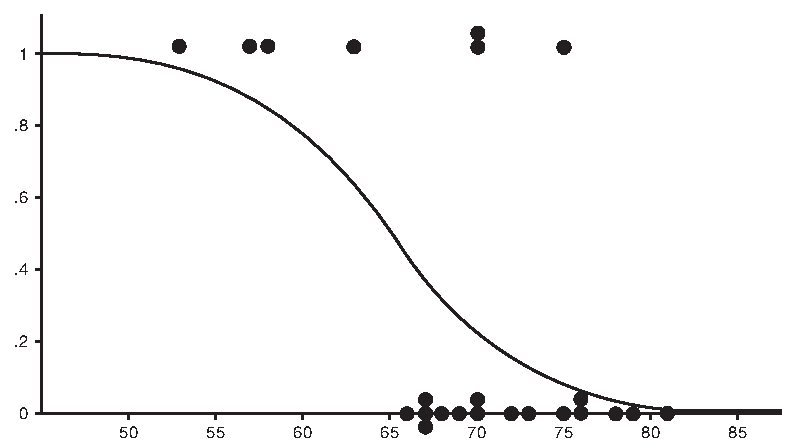
\includegraphics[width=.92\textwidth]{assets/chapter12/fig-12.3.1.pdf}
\caption{\autoref{tab:12.3.1}的数据及拟合的逻辑曲线}\label{fig:12.3.1}
\end{figure}
\sourcepageanchor{513}
到目前为止，假定在每个$x_i$值只观测一次Bernoulli试验的结果. 虽然经常如此，但很多情形会在每个$x$值处观测多个Bernoulli结果. 现在重新考察这一更一般情形的似然解.

设数据集中预测变量$x$有$J$个不同取值$x_1,\ldots,x_J$. 用$n_j$表示$x_j$处的Bernoulli观测数，$Y_j^*$表示这些$n_j$次观测中的成功数. 因而$Y_j^*\sim\operatorname{binomial}(n_j,\pi(x_j))$. 似然为\footnote{译注：原式第一项使用$x_i$而乘积下标为$j$，按定义应为$x_j$；还省略了不依赖参数的二项系数，故应理解为与似然成比例. 原式保留.}
$$L(\alpha,\beta\mid\boldsymbol y^*)=\prod_{j=1}^J\pi(x_i)^{y_j^*}(1-\pi(x_i))^{n_j-y_j^*}
=\prod_{j=1}^JF_j^{y_j^*}(1-F_j)^{n_j-y_j^*},$$
似然方程为
$$\begin{aligned}
0&=\sum_{j=1}^J(y_j^*-n_jF_j)\frac{f_j}{F_j(1-F_j)},\\
0&=\sum_{j=1}^J(y_j^*-n_jF_j)\frac{f_j}{F_j(1-F_j)}x_j.
\end{aligned}$$
既然用最大似然估计了逻辑回归参数，接下来就可利用MLE的渐近理论得到近似方差. 但必须以更一般的方式处理. \autoref{sec:10.1.3}曾利用信息数近似MLE的方差. 这里采用同一策略，但由于有两个参数，需要由以下$2\times2$矩阵给出的信息矩阵（information matrix）：
\begin{equation}\label{eq:12.3.9}
I(\theta_1,\theta_2)=\begin{pmatrix}
-\dfrac{\partial^2}{\partial\theta_1^2}\log L(\theta_1,\theta_2\mid\boldsymbol y)&
-\dfrac{\partial^2}{\partial\theta_1\partial\theta_2}\log L(\theta_1,\theta_2\mid\boldsymbol y)\\
-\dfrac{\partial^2}{\partial\theta_1\partial\theta_2}\log L(\theta_1,\theta_2\mid\boldsymbol y)&
-\dfrac{\partial^2}{\partial\theta_2^2}\log L(\theta_1,\theta_2\mid\boldsymbol y)
\end{pmatrix}.
\end{equation}
逻辑回归的信息矩阵为
\begin{equation}\label{eq:12.3.10}
I(\alpha,\beta)=\begin{pmatrix}
\sum_{j=1}^Jn_jF_j(1-F_j)&\sum_{j=1}^Jx_jn_jF_j(1-F_j)\\
\sum_{j=1}^Jx_jn_jF_j(1-F_j)&\sum_{j=1}^Jx_j^2n_jF_j(1-F_j)
\end{pmatrix},
\end{equation}
通常利用这一矩阵近似MLE $\hat\alpha,\hat\beta$的方差. 注意$I(\alpha,\beta)$的元素不依赖$Y_1^*,\ldots,Y_J^*$. 因而，在这种情形下，观测信息与信息相同.

\autoref{sec:10.1.3}使用近似\eqref{eq:10.1.7}，即$\operatorname{Var}(h(\hat\theta)\mid\theta)\approx[h'(\hat\theta)]^2/I(\hat\theta)$，其中$I(\cdot)$为信息数. 对信息矩阵不能完全照搬，而要先求逆，再用逆矩阵元素近似方差. 回顾$2\times2$矩阵的逆为
$$\begin{pmatrix}a&b\\c&d\end{pmatrix}^{-1}
=\frac1{ad-bc}\begin{pmatrix}d&-b\\-c&a\end{pmatrix}.$$
为得到近似方差，用MLE估计矩阵\eqref{eq:12.3.10}中的参数；方差估计$[\operatorname{se}(\hat\alpha)]^2$、$[\operatorname{se}(\hat\beta)]^2$就是$I(\hat\alpha,\hat\beta)$的逆矩阵的对角元素.

\enlargethispage{1pt}
\begin{example}[挑战者号数据续]\label{ex:12.3.2}
挑战者号数据所得估计量的估计信息矩阵为
$$\begin{aligned}
I(\hat\alpha,\hat\beta)&=\begin{pmatrix}
\sum_{j=1}^J\hat F_j(1-\hat F_j)&\sum_{j=1}^Jx_j\hat F_j(1-\hat F_j)\\
\sum_{j=1}^Jx_j\hat F_j(1-\hat F_j)&\sum_{j=1}^Jx_j^2\hat F_j(1-\hat F_j)
\end{pmatrix}\\
&=\begin{pmatrix}3.15&214.75\\214.75&14728.5\end{pmatrix},
\end{aligned}$$
\sourcepageanchor{514}
其中$\hat F_j=e^{\hat\alpha+\hat\beta x_j}/(1+e^{\hat\alpha+\hat\beta x_j})$，其逆为
$$I(\hat\alpha,\hat\beta)^{-1}=\begin{pmatrix}59.19&-.86\\-.86&.013\end{pmatrix}.$$
例如，似然渐近理论说明，大样本时$\hat\beta\pm z_{\alpha/2}\operatorname{se}(\hat\beta)$是$\beta$的近似$100(1-\alpha)\%$置信区间. 因而，挑战者号数据给出的95\%置信区间为
$$\beta\in-.243\pm1.96\times\sqrt{.013}\quad\Rightarrow\quad-.466\le\beta\le-.02,$$
支持$\beta<0$的结论.
\end{example}

这一模型中最常见的检验也许是假设$H_0:\beta=0$，因为和简单线性回归一样，这一假设表示预测变量与响应变量没有关系. 若$H_0$成立且样本量很大，Wald检验统计量$Z=\hat\beta/\operatorname{se}(\hat\beta)$近似服从标准正态分布. 因而，若$|Z|\ge z_{\alpha/2}$，可拒绝$H_0$. 也可用对数似然比检验统计量检验$H_0$：\footnote{译注：括号中第二项按对数似然比定义应为$\log L(\hat\alpha_0,0\mid\boldsymbol y^*)$，原文漏log，照录.}
$$-2\log\lambda(\boldsymbol y^*)=2[\log L(\hat\alpha,\hat\beta\mid\boldsymbol y^*)-L(\hat\alpha_0,0\mid\boldsymbol y^*)],$$
其中$\hat\alpha_0$是$\beta=0$时$\alpha$的MLE. 利用通常的二项分布论证（\autoref{exercise:12.20}），可证明$\hat\alpha_0=\sum_{i=1}^ny_i/n=\sum_{j=1}^Jy_j^*/\sum_{j=1}^Jn_j$.\footnote{译注：右边估计的是共同成功概率$p$，而截距满足$\alpha_0=\log(p/(1-p))$，所以应对所给比例取logit. 原式保留.} 因此，在$H_0$下，$-2\log\lambda$近似服从$\chi_1^2$分布，若$-2\log\lambda\ge\chi_{1,\alpha}^2$，可在水平$\alpha$拒绝$H_0$.

这里只介绍了最简单的逻辑回归与广义线性模型. 更多内容可见\hyperref[bib:source1]{Agresti（1990）}等标准教材.
